\newpage
\section{Definición del problema y análisis de requisitos}
\label{cap:analisis_requisitos}

La ingeniería de requisitos constituye una fase crítica en el ciclo de vida del desarrollo de sistemas, estableciendo el marco de referencia técnico que guiará el diseño y la implementación. En este capítulo se formaliza la especificación del sistema propuesto, delimitando las restricciones operativas, definiendo los actores involucrados y detallando los requisitos funcionales y no funcionales bajo directrices estandarizadas de ingeniería de software \cite{iso29148}.

\subsection{Restricciones y factores limitantes}
El desarrollo e implantación del prototipo están sujetos a un conjunto de restricciones físicas, tecnológicas y temporales que condicionan la arquitectura final:
\begin{itemize}
    \item \textbf{Restricciones de conectividad y latencia:} el sistema opera sobre una red local aislada para garantizar la resiliencia frente a caídas del servicio de Internet (arquitectura \textit{offline-first}). Esto exige que el servidor central y los sensores compartan el mismo dominio de difusión (dominio de \textit{broadcast}) y estén sometidos a una estricta política de red.
    \item \textbf{Restricciones ambientales y volumétricas:} la fiabilidad de la telemetría espacial está supeditada a la geometría de la habitación y a la existencia de línea de visión electromagnética directa entre el radar de ondas milimétricas y los sujetos, limitando las posiciones de instalación viables para evitar zonas de sombra acústica.

    \item \textbf{Restricciones de hardware y procesamiento:} la gestión centralizada central se ejecuta sobre un microordenador Raspberry Pi 4 de recursos finitos. Esto impone una limitación directa sobre la complejidad computacional algorítmica y exige un control estricto sobre el uso de la memoria RAM y el desgaste de la unidad de almacenamiento.
    \item \textbf{Restricciones de infraestructura de red:} el sistema exige cobertura ininterrumpida de red inalámbrica IEEE 802.11 (Wi-Fi) en la banda de 2.4 GHz para la transmisión de la telemetría a través de la API local de los nodos distribuidos, requiriendo un nivel de señal (RSSI) estable para evitar la pérdida de eventos lógicos.
\end{itemize}

\begin{figure}[H]
    \centering
    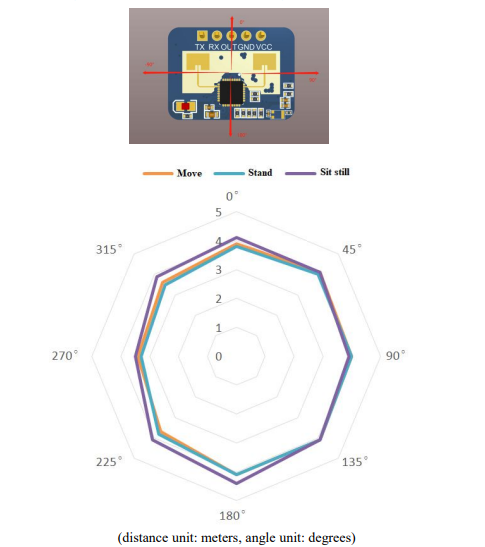
\includegraphics[width=0.7\textwidth]{Img/diagrama_rango.png}
    \caption{Campo de visión volumétrica del sensor FMCW. Adaptado de \cite{datasheetHLKLD2410}.}
    \label{fig:campo_vision_radar}
\end{figure}

\subsection{Identificación de actores del sistema}
Para el modelado lógico de los casos de uso, se identifican los siguientes actores que interactúan de forma directa o indirecta con la infraestructura:
\begin{itemize}
    \item \textbf{Usuario habitual:} actor principal y pasivo. Representa a la persona física que habita el entorno monitorizado. Su interacción consiste en realizar rutinas cotidianas (estudiar, dormir, salir) sin requerir la emisión de comandos explícitos al sistema.
    \item \textbf{Administrador del sistema:} actor activo con privilegios elevados. Encargado del mantenimiento de la infraestructura, el acceso al panel de control analítico, la calibración de los umbrales de sensibilidad de los sensores y la auditoría de los registros de ejecución.
    \item \textbf{Motor de contexto (actor lógico):} entidad de software autónoma que procesa la telemetría entrante, ejecuta los algoritmos de fusión de datos y emite las órdenes de actuación sobre el entorno físico.
\end{itemize}

\begin{figure}[H]
    \centering
    
\begin{tikzpicture}[
        actor/.style={circle, draw=black!80, fill=blue!10, thick, minimum size=1.2cm, align=center, font=\small\sffamily},
        system/.style={rectangle, draw=red!80, fill=white, thick, minimum width=6.5cm, minimum height=6cm, rounded corners},
        usecase/.style={ellipse, draw=black!80, fill=yellow!20, thick, minimum width=3.5cm, minimum height=1.2cm, align=center, font=\footnotesize\sffamily},
        arrow/.style={->, >=stealth, thick, color=black!70}
    ]
        % Sistema
        \node[system] (sys) at (0,0) {};
        \node[anchor=north, font=\bfseries] at (sys.north) {Sistema Domótico};

        % Casos de uso
        \node[usecase] (cu1) at (0, 1.8) {Calibración y\\Auditoría};
        \node[usecase] (cu2) at (0, 0) {Generación de\\Telemetría};
        \node[usecase] (cu3) at (0, -1.8) {Inferencia de\\Estados y Actuación};

        % Actores
        \node[actor] (admin) at (-4.5, 1.8) {Admin.};
        \node[actor] (user) at (-4.5, -0.5) {Usuario\\habitual};
        \node[actor, fill=green!10] (engine) at (4.5, -1.5) {Motor de\\Contexto};

        % Conexiones
        \draw[arrow] (admin) -- (cu1);
        \draw[arrow] (user) -- (cu2);
        \draw[arrow] (engine) -- (cu3);
        
        \draw[arrow, dashed] (cu2) -- (engine);
    \end{tikzpicture}
    \caption{Diagrama de casos de uso y actores del sistema.}
    \label{fig:casos_uso_actores}
\end{figure}

\subsection{Requisitos funcionales (RF)}
Los requisitos funcionales describen las operaciones y comportamientos específicos que el sistema debe ser capaz de ejecutar en su entorno de producción.
\begin{itemize}
    \item \textbf{RF-01: Monitorización espacial continua.} El sistema debe detectar la ocupación volumétrica con resolución submilimétrica, diferenciando de manera inequívoca los estados de movimiento dinámico y reposo biométrico absoluto.
    \item \textbf{RF-02: Adquisición de telemetría ambiental.} El sistema debe registrar variables de luminosidad ambiental e índices termohigrométricos para nutrir la matriz de contexto.
    \item \textbf{RF-03: Inferencia algorítmica de estados.} El servidor central debe procesar las entradas sensoriales para asignar unívocamente un estado lógico continuo a la estancia (ocio, estudio, durmiendo, ausente).
    \item \textbf{RF-04: Actuación física proactiva.} El sistema debe controlar la apertura y cierre de relés de estado sólido para la iluminación en función de reglas paramétricas asociadas a la productividad (gestión de tiempos ininterrumpidos) y la ergonomía visual.
    \item \textbf{RF-05: Emisión de notificaciones y alertas.} El sistema debe poseer la capacidad de notificar eventos críticos o advertencias de inactividad prolongada al dispositivo móvil del Administrador.
\end{itemize}

\subsection{Requisitos no funcionales (RNF)}
Los requisitos no funcionales establecen los criterios de calidad, las métricas de rendimiento y las restricciones de diseño arquitectónico.
\begin{itemize}
    \item \textbf{RNF-01: Operatividad perimetral aislada (\textit{edge computing}).} El procesamiento algorítmico, las máquinas de estado y el registro en bases de datos deben ejecutarse estrictamente en la red local, garantizando la operatividad sin salida a internet.
    \item \textbf{RNF-02: Baja latencia transaccional.} El tiempo de respuesta entre el registro de un evento físico (ej. cruce del umbral de la puerta) y la ejecución de la acción en el actuador (ej. conmutación del relé) no debe exceder de 1000 milisegundos.
    \item \textbf{RNF-03: Resiliencia ante caídas de red.} El servidor central debe identificar la desconexión abrupta de cualquier nodo sensor y aplicar un protocolo de contingencia mediante el mecanismo de supervisión activa (\textit{keepalive}) de la API nativa de ESPHome.
    \item \textbf{RNF-04: Tolerancia a fallos lógicos.} El motor de contexto debe implementar reglas condicionales redundantes para rectificar falsos positivos de hardware y forzar transiciones de estado seguras (ej. auto-armado por inactividad).
\end{itemize}

\subsection{Consideraciones normativas, de seguridad y privacidad}
El tratamiento de datos derivados de constantes biométricas (frecuencia respiratoria) y rutinas de presencia exige el cumplimiento estricto del paradigma de privacidad desde el diseño (\textit{Privacy by Design}) \cite{cavoukian2009privacy}. Al confinar el almacenamiento de las series temporales al entorno perimetral de la propia vivienda y prescindir de plataformas de terceros, el diseño cumple inherentemente con el principio de minimización de exposición de datos. 

\begin{figure}[H]
    \centering
    
\begin{tikzpicture}[
        node distance=1.5cm and 1.8cm,
        box/.style={rectangle, draw=black!80, fill=blue!5, thick, minimum width=2.5cm, minimum height=1.5cm, align=center, rounded corners},
        cloud/.style={ellipse, draw=black!80, fill=gray!20, thick, minimum width=3cm, minimum height=2cm, align=center},
        firewall/.style={rectangle, draw=red, fill=red!20, thick, minimum width=0.5cm, minimum height=2cm}
    ]
        % Nodos locales
        \node[box] (sensor) {Nodos Sensores\\(ESP32 + Radar)};
        \node[box, right=of sensor] (broker) {Servidor central Local\\(Raspberry Pi)};
        \node[box, below=of sensor] (actuator) {Actuadores\\(Relés)};
        
        % Internet y Cloud
        \node[firewall, right=0.8cm of broker] (fw) {};
        \node[cloud, right=0.8cm of fw] (internet) {Internet /\\Cloud Externo};

        % Etiquetas
        \node[anchor=south, font=\bfseries\small, color=red] at ([yshift=0.3cm]fw.north) {Aislamiento (WPA3)};

        % Conexiones
        \draw[<->, >=stealth, thick, color=black!70] (sensor) -- node[above, font=\footnotesize] {API nativa} (broker);
        \draw[<->, >=stealth, thick, color=black!70] (broker) |- node[right, font=\footnotesize] {API nativa} (actuator);
        
        % Bloqueo
        \draw[->, >=stealth, thick, red, dashed] (broker) -- (fw);
        \draw[->, >=stealth, thick, red, dashed] (fw) -- (internet);
        \node[red, font=\Large\bfseries] at (fw) {X};
        
        % Caja perimetral dinámica
        \draw[thick, dashed, color=blue, rounded corners] 
            ([xshift=-0.5cm, yshift=0.6cm]sensor.north west) 
            rectangle 
            ([xshift=0.5cm, yshift=-0.5cm]broker.south east |- actuator.south);
            
        \node[color=blue, font=\bfseries, anchor=south west] 
            at ([xshift=-0.5cm, yshift=0.6cm]sensor.north west) {Red Local (Edge)};

    \end{tikzpicture}
    \caption{Arquitectura de red aislada garantizando la Privacidad desde el Diseño.}
    \label{fig:edge_privacy}
\end{figure}

En el ámbito de la seguridad de las telecomunicaciones, el blindaje de la infraestructura reside en la robustez criptográfica del estándar de autenticación de la red inalámbrica de área local (WPA2/WPA3). Esto previene ataques de inyección de telemetría y bloquea la intercepción pasiva de las comunicaciones de la API local por agentes externos al perímetro.

\subsection{Matriz de trazabilidad}
La trazabilidad metodológica asegura que cada requisito técnico del diseño responde directamente a un objetivo formalizado del proyecto. La Tabla \ref{tab:trazabilidad} correlaciona los Objetivos Específicos (OE), detallados en el Capítulo 1, con los requisitos funcionales y no funcionales aprobados para el sistema.

\begin{table}[H]
    \centering
    \caption{Matriz de trazabilidad entre objetivos específicos y requisitos del sistema.}
    \label{tab:trazabilidad}
    \begin{tabular}{|l|c|c|}
        \hhline{|-|-|-|}
        \rowcolor[gray]{0.9} 
        \parbox[c]{5cm}{\vspace{0.3cm}\centering \textbf{Objetivo Específico (OE)}\vspace{0.3cm}} & \parbox[c]{4cm}{\centering \textbf{Requisitos Func. (RF)}} & \parbox[c]{4cm}{\centering \textbf{Req. No Func. (RNF)}} \\ \hhline{|-|-|-|}
        \parbox[c]{5cm}{\vspace{0.3cm}\centering OE-1: Diseño de hardware distribuido\vspace{0.3cm}} & RF-01, RF-02 & RNF-01 \\ \hhline{|-|-|-|}
        \parbox[c]{5cm}{\vspace{0.3cm}\centering OE-2: Telemetría avanzada\vspace{0.3cm}} & RF-01, RF-02 & RNF-02 \\ \hhline{|-|-|-|}
        \parbox[c]{5cm}{\vspace{0.3cm}\centering OE-3: Motor de contexto\vspace{0.3cm}} & RF-03 & RNF-01, RNF-04 \\ \hhline{|-|-|-|}
        \parbox[c]{5cm}{\vspace{0.3cm}\centering OE-4: Automatización y seguridad\vspace{0.3cm}} & RF-04, RF-05 & RNF-02, RNF-03 \\ \hhline{|-|-|-|}
        \parbox[c]{5cm}{\vspace{0.3cm}\centering OE-5: Validación e integración\vspace{0.3cm}} & RF-03 & RNF-03, RNF-04 \\ \hhline{|-|-|-|}
    \end{tabular}
\end{table}